% Hier wird der theoretische Teil vorgenommen. 

\chapter{Clean Architecture}

Dieses Kapitel beschäftigt sich mit dem Stand der Technik, der Einordnung dieser Arbeit in die Literatur 
und den Grundlagen der Konzeption. Hierfür sind zunächst 
die Aufgabenkategorien der Computer-Vision zu vergleichen, um eine geeignete für das gegebene Problem finden zu können.
Ebenso wird für verschiedene state-of-the-art Aktivierungsfunktionen und Ähnlichkeitsmaße verfahren, 
sodass später geeignete ausgewählt und diskutiert werden können. Daraufhin sind 
die Vorteile einiger relevanter Architekturkomponenten zu betrachten und einige 
state-of-the-art Klassifikationsmodelle des ImageNet-Datensatzes, welche ggf. 
als vortrainierte Bestandteile der späteren Architektur verwendet werden können, 
was genauer im Abschnitt \textit{Transfer-Learning mit U-Net} betrachtet ist. 
Schließlich wird der aktuelle Stand bei der verwandten Domäne der Straßenerkennung 
aus Luftaufnahmen untersucht.

\section{Aufgabenkategorien} \label{sec:aufgabenkategorien}
Im Bereich der Computer Vision gibt es verschiedene Problemstellungen, die unterschiedlich gelöst werden können.
Die einzelnen Lösungsansätze werden jeweils einer Aufgabenkategorie zugeordnet.
Nachfolgend wird ein Überblick über die Kategorien \textit{Klassifizierung}, \textit{Object Detection} und \textit{Image Semantic Segmentation} gegeben.
Eine Visualisierung ist in \autoref{fig:categories} gegeben.
Die aufgeführten Kategorien nehmen in der genannten Reihenfolge in ihrer Komplexität zu.

\begin{itemize}
	\item \textit{Klassifizierung:}
	Eine reine Klassifizierung ist die einfachste Lösungskategorie. 
	Es soll lediglich erkannt werden, welche Klasse in einem Bild enthalten ist.
	Die Lokalität des erkannten Objektes wird vernachlässigt, wichtiger ist die Zuordnung zu einer Klasse.
	Dies lässt sich auch entsprechend auf die Erkennung von mehreren Klassen erweitern.
	
	\item \textit{Object Detection:}
	Eine Erweiterung der Klassifizierung um die Lokalität des erkannten Objektes wird \textit{Image Localization} genannt.
	Für mehrere Objekte wird der Begriff Object Detection verwendet.
	Die Darstellung erkannter Objekte wird über Bounding Boxes realisiert, welche die Objekte jeweils umschließen.

	\item \textit{Image Semantic Segmentation:}
	Die bei der Object Detection verwendeten Bounding Boxes geben keine Rückschlüsse auf die konkrete Form der Klasse.
	Je nach Lage des Objektes kann nur ein Bruchteil der Bounding Box von der erkannten Klasse gefüllt sein.
	Abhilfe schafft die Verwendung einer pixelweisen Maske anstelle einer Bounding Box, das Objekt kann von seiner Umgebung abgegrenzt werden.
	Zusätzlich kann gefordert werden, dass einzelne Instanzen verschiedener Objekte unterschieden werden sollen.
	Diese Forderung wird dann \textit{Instance Segmentation} genannt \cite{Sharma.21.08.2019}.
\end{itemize}

\begin{figure}
	\centering
	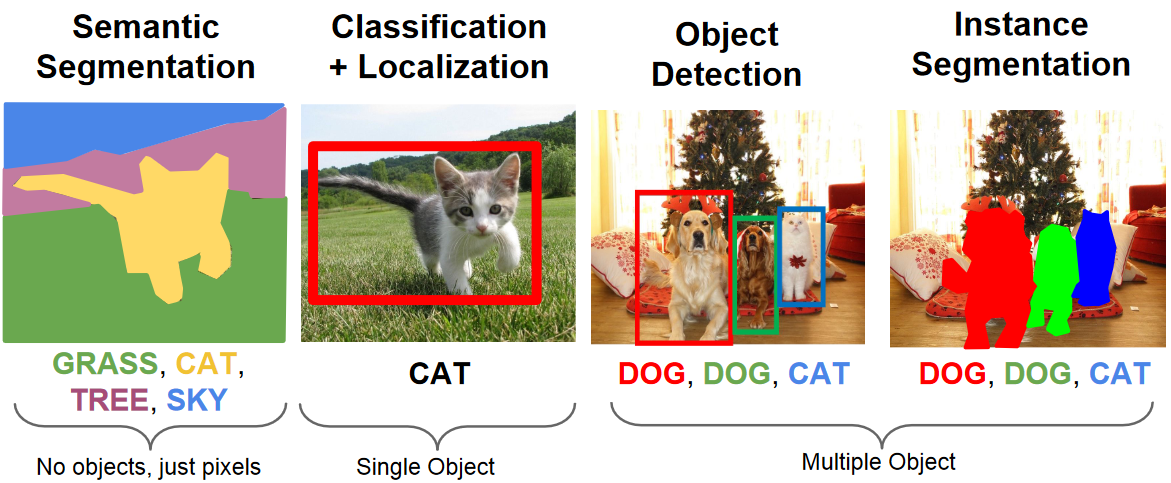
\includegraphics[width=0.8\textwidth]{Bilder/categories.png} 
	\caption{Verschiedene Aufgabenkategorien \cite{.10.11.2022}.}
	\label{fig:categories}
\end{figure} 

\section{Aktivierungsfunktionen} \label{sec:activation}

Im Folgenden wird der Stand der Technik für Aktivierungsfunktionen in \ac{ML}-Modellen dargelegt,
hierzu werden einige Funktionen kurz vorgestellt und deren Vor- und Nachteile bewertet. 
Die besprochenen Funktionen sind dargestellt in \autoref{fig:activation}.

\subsection{Sigmoid}

Die \textit{Sigmoid}-Funktion bildet die Eingabe auf einen Wert im Intervall $(0;1)$ ab und wird durch \autoref{eq:sigmoid} beschrieben.
Der Vorteil hier ist, dass Aktivierungen nie groß werden können, wodurch einzelne Neuronen nicht den Gradienten dominieren können und 
eine fortlaufende Normalisierung durchgeführt wird. Die Probleme hingegen sind, dass die Funktion eher aufwendig zu berechnen ist 
und dass die Ableitung für betragsmäßig größere Werte verschwindet. Hierdurch kann es zum \textit{Vanishing-Gradient-Problem} kommen, wobei 
Neuronen in den flacheren Schichten eines neuronalen Netzes kaum noch geupdated werden \cite[S.~191--192]{Goodfellow.2016} 
\begin{align}
	\label{eq:sigmoid} Sigmoid(z) = \frac{1}{1+e^{-z}}~.
\end{align} 

\subsection{\acf{ReLU}}

Die \textit{\acf{ReLU}} ist eine Aktivierungsfunktion, welche durch \autoref{eq:relu} ausgedrückt wird. 
\ac{ReLU} ist inzwischen der de-facto Standard von Aktivierungsfunktionen in den verborgenen Schichten eines Deep-Learning-Modells.
Dies liegt vor allem daran, dass das Vanishing-Gradient-Problem adressiert wird. Allerdings hat \ac{ReLU} das Problem, 
dass Neuronen auf $0$ gesetzt werden, wodurch sie kein Gradienten-Update mehr erhalten und dauerhaft genullt bleiben 
und somit nichts mehr zum Netzwerk beitragen - die Neuronen sterben. Das Problem wird \textit{Dying-\ac{ReLU}-Problem} genannt \cite[S.~189--191]{Goodfellow.2016} 
\begin{align}
	\label{eq:relu} ReLU(z) = \begin{cases} 
		z & z > 0 \\
		0 & z \leq 0 
	\end{cases}~.
\end{align} 

\ac{ReLU} erzielt eine höhere Inferenz- und Trainingsgeschwindigkeit bei gleicher oder besserer Performanz, 
als Sigmoid. Dies liegt zum einen an der Verbesserung des Vanishing-Gradient-Problems und zum anderen an der 
simpleren und damit leichter zu berechnenden Funktion \cite[S.~226]{Goodfellow.2016}.

\subsection{\acf{ELU}}

Die \textit{\acf{ELU}} ist eine Aktivierungsfunktion, die das Dying-\ac{ReLU}-Problem adressieren soll. 
Ausgedrückt wird die Funktion durch \autoref{eq:elu}. Die negative Komponente lässt zu, dass Neuronen nicht 
von einem Satz auf $0$ zurückkommen können, und weiterhin etwas zur Zielfunktion beitragen können. Außerdem ist die mittlere 
Aktivierung näher an $0$ als bei \ac{ReLU}, was zur Folge hat, dass das Training schneller konvergiert \cite{Clevert.23112015}
\begin{align}
	\label{eq:elu} ELU(z) = \begin{cases} 
		z & z > 0 \\
		\alpha \cdot (e^z - 1) & z \leq 0 
	\end{cases} ~.
\end{align}

Sowohl \ac{ReLU} als auch \ac{ELU} haben das Problem, dass Aktivierungen beliebig groß werden können, 
wodurch einige wenige Neuronen den Gradienten dominieren können, was zu langsamen Training und suboptimaler Performanz führen kann. 
\begin{figure}
	\centering
	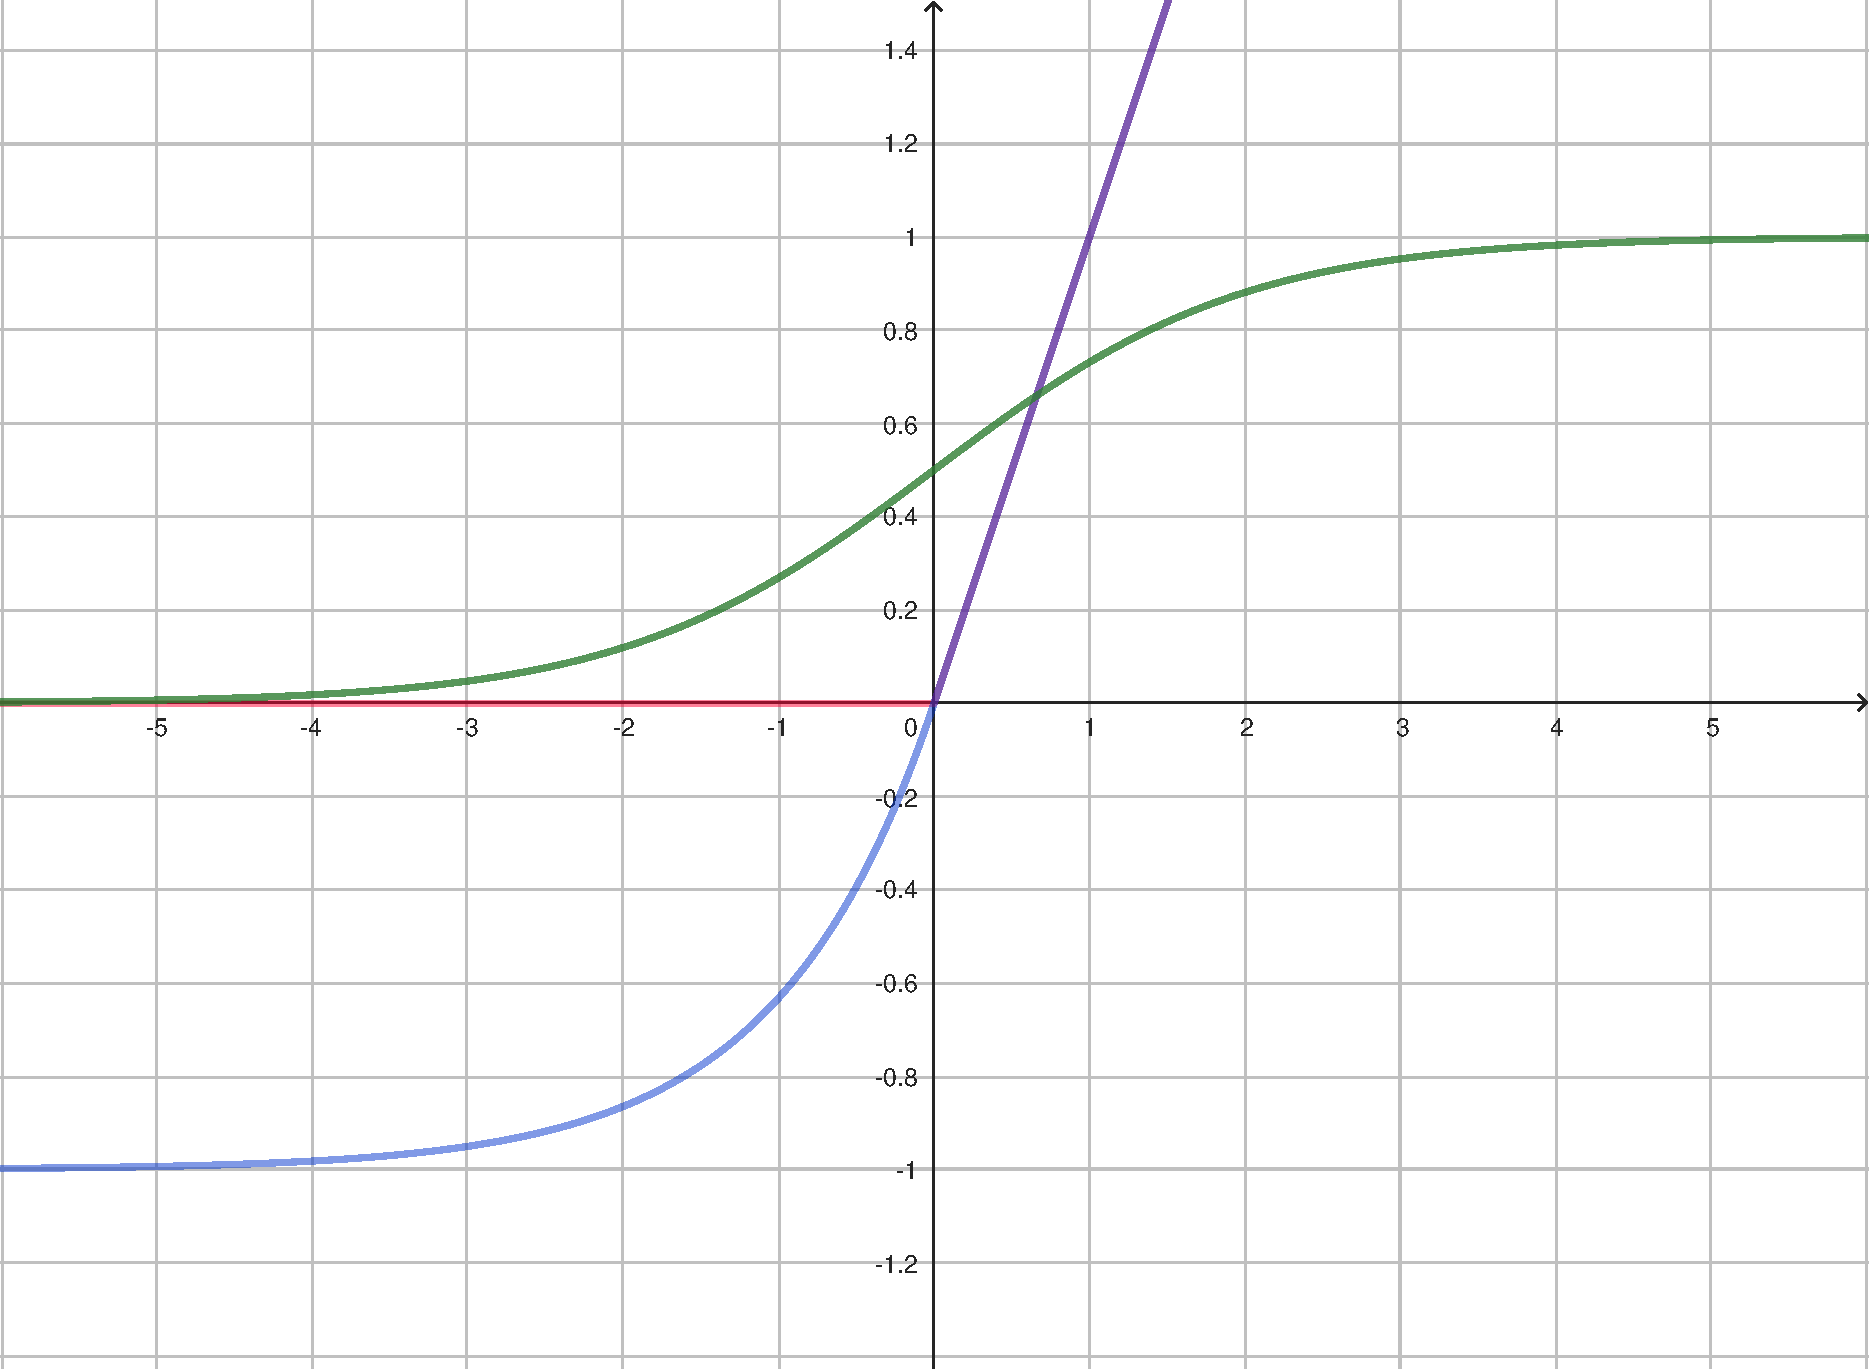
\includegraphics[width=0.8\textwidth]{Bilder/activation-geogebra-export.pdf} 
	\caption{Verschiedene Aktivierungsfunktionen. Grün: Sigmoid. Rot: \ac{ReLU}. Blau: \ac{ELU} mit $\alpha = 1$.}
	\label{fig:activation}
\end{figure} 


\section{Ähnlichkeitsmaße} \label{sec:evaluation-metrics}

Im Folgenden sollen Ähnlichkeitsmaße zwischen Mengen, insbesondere 
solche, die als Kostenfunktion bzw. Bewertungsmetrik für einen binären 
Klassifikator verwendet werden können, untersucht werden. Hierzu wird zunächst Cross-Entropy betrachtet,
gefolgt von dem Dice- bzw. F-Maß. Weiter werden \ac{IoU} und das darauf aufbauende Quality-Maß betrachtet.

\subsection{\acf{BCE}}

Die \textit{Cross-Entropy} (bzw. dt. \textit{Kreuzentropie}) ist ein Maß des Unterschieds zweier
Wahrscheinlichkeitsdistributionen. Im Spezialfall einer binären Wahrscheinlichkeitsvariable 
kann die Cross-Entropy zur \textit{\acf{BCE}} spezialisiert werden, um auf ein binäres 
Klassifikationsproblem angewandt zu werden. 
\autoref{eq:bce} zeigt die Kalkulation von \ac{BCE}, wobei $p \in [0;1]$ die Prediction 
eines binären Klassifikators und $y \in \{0,1\}$ der Wert des Labels darstellen
\begin{align}
	\label{eq:bce} BCE = -[p \cdot \log(y) + (1-p) \cdot \log(1-y) ]~.
\end{align} 
Um über $n$ Prediction-Label-Paare $(p_i; y_i)$ den \ac{BCE} zu berechnen, wird das arithmetische Mittel nach
\autoref{eq:bce-mean} gebildet \cites[S.~82]{Cybenko.1999}[S.~57--59]{Murphy.2012}
\begin{align}
	\label{eq:bce-mean} BCE = -\frac{1}{n}\sum_{i = 1}^{n}[p_i \cdot \log(y_i) + (1-p_i) \cdot \log(1-y_i) ]~.
\end{align}

Im Sinne einer differenzierbaren Kostenfunktion im Kontext von \ac{ML} sind \ac{BCE},
\textit{negative Log-Likelihood} und \textit{Logistic-Regression} synonym \cite[S.~249]{Murphy.2012}. 

Aus \autoref{eq:bce-mean} geht hervor, warum \ac{BCE} gut geeignet für Klassifikationsprobleme ist.
Im Gegensatz zum mittleren absoluten Fehler, bei dem ein Fehler linear eingeht, und zum mittleren quadratischen Fehler,
bei dem ein Fehler quadratisch eingeht, geht ein Fehler bei \ac{BCE} exponentiell ein. 
Ein größerer Fehler wiegt also exponentiell stärker als ein kleinerer Fehler. 
Hierdurch werden die Fehler pro Datenpunkt und Klasse sehr klein, 
wodurch gute Performance und gute Generalisierung bei \ac{ML}-Modellen erreicht werden können. \\

Bei stark ungleichmäßiger Klassenverteilung kann es jedoch dazu kommen, 
dass die unterrepräsentierte Klasse kaum noch geschätzt wird, 
da der Fehler einer falsch geschätzten überrepräsentierten Klasse zu stark bestraft wird.
Dadurch lernt der Algorithmus, die unterrepräsentierte Klasse kaum zu schätzen.
Eine Abhilfe dagegen schafft eine Gewichtung der unterschiedlichen Klassen \cite[S.~4]{Ronneberger.18052015}.

\subsection{Dice- und F-Maß}

Das \textit{Dice-}, oder auch \textit{Sorensen-Dice-}Maß $D$ wurde 1945 bzw. 1948 erstmals vorgestellt und genutzt, um die Ähnlichkeit zweier botanischer Stichproben zu ermitteln. Verallgemeinert auf diskrete Mengen $X$, $Y$ kann deren Ähnlichkeit nach Dice $D$ beschrieben werden durch \autoref{eq:roll-coeff}. Es gilt $D \in [0; 1]$ \cites[S.~33]{Srenson.1948}[S.~297]{Dice.1945}
\begin{align}
	\label{eq:roll-coeff} D = \frac{2 \cdot | X \cap Y |}{2 \cdot | X \cap Y | + |Y \setminus X| + |X \setminus Y|}
	=\frac{2 \cdot | X \cap Y |}{|X| + |Y|} ~.
\end{align} 

Angewandt auf boolesche Mengen und binäre Klassifikatoren ist das Dice-Maß gleich dem $F_1$-Maß, das ein Maß für die Qualität eines statistischen Tests darstellt. Dafür sei $X$ nun die Menge der positiven Elemente und $Y$ die Menge der als positiv eingestuften Elemente. Dann ist die \textit{Genauigkeit} oder auch \textit{Precision} gegeben durch
\begin{align}
	\label{eq:precision} precision = \frac{|X \cap Y|}{|Y|}~,
\end{align}
der Anteil der richtig eingestuften Elemente an allen positiv eingestuften Elementen und die \textit{Trefferquote} oder auch \textit{Recall} gegeben durch
\begin{align}
	\label{eq:recall} recall = \frac{|X \cap Y|}{|X|}~,
\end{align}
der Anteil der richtig eingestuften Elemente an allen positiven Elementen. \\
Das F-Maß, bzw. genauer das $F_1$-Maß, ist dann gegeben durch das harmonische Mittel aus Precision und Recall, wobei $tp$ die Anzahl von wahr-positiven, $fp$ die Anzahl von falsch-positiven und $fn$ die Anzahl von falsch-negativen Elementen ist \cite{YutakaSasaki.2007}:
\begin{align}
	\label{eq:f1} F_{1} = \frac{2\cdot precision \cdot recall}{precision + recall} = \frac{2\cdot tp}{2 \cdot tp + fp + fn}~.
\end{align}
Precision und Recall können mit einem Faktor $\alpha$ unterschiedlich zueinander gewichtet werden, um mit $F_{\alpha}$ unterschiedliche Aspekte zu fokussieren. 

Das Dice-, bzw. $F_{\alpha}$-Maß kann leicht für eine differenzierbare Kostenfunktion genutzt werden mit Dice-Loss $D_{L}(X, Y) = 1 - D(X,Y)$, bzw. $F_{\alpha}$-Loss $F_{\alpha L}(X,Y) = 1 - F_{\alpha}(X,Y)$. 


\subsection{\acf{IoU}}

Die \textit{\acf{IoU}-} bzw. \textit{Jaccard-Ähnlichkeitsmetrik} ist ein weit verbreitetes Maß zur Bestimmung der Ähnlichkeit zwei diskreter Mengen. Hierzu seien $X$ und $Y$ diskrete Mengen. Dann ist die $IoU$ gegeben durch 
\begin{align}
	\label{eq:iou} IoU = \frac{|X\cap Y|}{|X \cup Y|} = \frac{| X \cap Y |}{| X \cap Y | + |Y \setminus X| + |X \setminus Y|}~.
\end{align} 
Für ein binäres Klassifikationsproblem lässt sich die $IoU$ ausdrücken durch 
\begin{align}
	\label{eq:iou-binary} IoU = \frac{tp}{tp + fp + fn}~,
\end{align}
wobei $tp$, $fp$, $fn$ wie in \autoref{eq:f1} \cite{Fletcher.2018}. 

Auffällig ist die Ähnlichkeit zum Dice- bzw. $F_{1}$-Maß. Es ist allerdings anzumerken, dass bei Dice/$F_1$ die $tp$, also die wahr-positiven, stärker gewichtet werden, als bei der \ac{IoU}. Die augenscheinliche Ähnlichkeit lässt sich durch die Beziehungen
\begin{align}
	\label{eq:roll-iou} IoU = \frac{D}{2 - D} \\
	D = \frac{2 \cdot IoU}{1 + IoU} ~,
\end{align}
beschreiben.
Im Gegensatz zur \ac{IoU} wird beim Dice-Maß eine höhere Gewichtung auf die wahr-positiven Elemente 
gelegt.

\subsection{Quality}

Bei der \textit{Quality} handelt es sich um eine gepufferte Form des \ac{IoU},
die toleranter bezüglich der Lokalität der Elemente der verglichenen Mengen, oder konkreter,
der Pixel einer semantischen Segmentierung, ist, 
wobei für dieselbe Eingabe $Quality \geq IoU$; $Quality \in [0;1]$ gilt, abhängig von der Puffergröße. 
Die Quality wird analog zur \ac{IoU} über eine gepufferte Precision - die \textit{Correctness} - 
und über einen gepufferten Recall - die \textit{Completeness} - berechnet. Insbesondere werden einige Elemente, 
die zuvor als $fp$ und $fn$ eingeordnet wurden, hiermit zu $tp$ konvertiert. \\
Die Quality soll einige Probleme der \ac{IoU} beheben, um ein Ähnlichkeitsmaß darzustellen, 
was näher an der praktischen und vom Menschen wahrgenommen Leistung eines \ac{ML}-Modells zur semantischen Segmentierung liegt.
So soll relativiert werden, dass vor allem im Randbereich einer Segmentierung einzelne abweichende Pixel
nicht als falsch anerkannt werden, sodass die Segmentierung im Großen und Ganzen als richtig anerkannt wird \cite{ChristianWiedemann.1998}. 

In dieser Arbeit für den Spezialfall von semantischer Segmentierung wird die Quality wie folgt berechnet: 
Sei $P$ die Prediction der Segmentierungsmaske für ein Eingabebild, $Y$ die tatsächliche Segmentierungsmaske (Ground-Truth / Label)
und $P, Y \in \{0, 1\}^{w \times h}$, wobei $w$ und $h$ die Breite und Höhe des Eingabebildes darstellen.
Die Einträge mit Wert eins von $P$ und $Y$ sind positiv, die Einträge mit Wert null negativ. Einträge repräsentieren Pixel.
$B$ sei die Puffergröße in Pixeln. \\
Zunächst sei die Hilfsfunktion $dilate_B: \{0,1\}^{w \times h} \mapsto \{0,1\}^{w \times h}$ definiert als 
\newcommand{\norm}[1]{\left\lVert#1\right\rVert}
\begin{align}
	\label{eq:dilate} dilate_B(A) = \left( \begin{cases} 
		1 & \exists a_{kl} \in A: a_{kl} = 1 \land \norm{
			\begin{pmatrix} k \\ l \end{pmatrix} - \begin{pmatrix} i \\ j \end{pmatrix} }_2 \leq B \\
		0 & else 
	\end{cases} \right)_{ij}~.
\end{align}
Die Funktion $dilate_B$ bildet eine Matrix auf eine weitere derselben Ordnung ab, 
sodass alle Einträge gleich eins sind, die in der Eingabematrix eins sind. Zusätzlich sind alle Einträge eins, 
die im Umkreis von $B$ Pixel um eine Eins in der Eingabematrix liegen. Somit werden die positiven 
Pixel der Eingabematrix um die Bufferzone erweitert.  \\
Damit lassen sich die gepufferten, fehlertoleranteren wahr-positiv $tp_B$, falsch-positiv $fp_B$ und 
falsch-negativ $fn_B$ Werte berechnen: 
\begin{align}
	\label{eq:buffering} {tp}_B = \norm{dilate_{B}(Y) \odot P}_{1,1} , \\
	fn_B = \norm{Y - (Y \odot dilate_{B}(P))}_{1,1} , \\
	{fp}_B = \norm{P}_{1,1} - {tp}_B .
\end{align}
Beispielhaft und intuitiv dargestellt für $tp_B$: Es sollen auch alle Eins-Pixel als wahr-positiv aufgefasst werden,
die leicht von der Ground-Truth abweichen, also sich noch in der Pufferzone befinden. 
Hierfür wird die Pufferzone um die Ground-Truth $Y$ gelegt und das Hadamard-Produkt mit der Predicition $P$ gebildet.
Da alle Matritzen als Einträge nur 0 oder 1 enthalten, findet durch das Hadamard-Produkt eine Art Verundung statt, 
sodass im Produkt nur Einträge eins sind, die in beiden Matritzen eins sind. Der Rest ist null. 
Durch die zuvor durchgeführte Pufferung mit $dilate_B$ sind allerdings auch Einträge gleich eins, die in $Y$ 
zuvor null waren. Hierdurch besitzt das Hadamard-Produkt mehr Einträge mit eins, als bei der Berechnung der \ac{IoU}.
Diese Zahl ist genau um die Anzahl an positiven Pixeln aus $P$ größer, die in der Pufferzone liegen. 
Schließlich wird mit der $1,1$-Höldernorm für Matritzen die Anzahl an Einsen gezählt, was dann $tp_B$ ergibt. \\
Die Formel für die Quality ist analog zur \ac{IoU}, bis auf die Verwendung der jeweils gepufferten Variablen:
\footnote{\autoref{code:quality} zeigt die dazugehörige Python-Implementation.}
\begin{align}
	\label{eq:quality} quality = \frac{tp_B}{tp_B + fp_B + fn_B} ~.
\end{align}

\section{Architekturkomponenten}

Im Folgenden werden verschiedene Architekturkomponenten diskutiert, die im \ac{ML} allgemein 
bzw. bei semantischer Segmentierung im Speziellen verwendet werden. Hierzu werden zunächst Dropout-Layer 
und Batch-Normalization-Layer begutachtet und dann die U-Net-Architektur zur semantischen Segmentierung vorgestellt. 

\subsection{Dropout} \label{sec:architekturkomponenten:dropout}

\textit{Dropout} ist eine ressourcenschonende Regularisierungstechnik für \ac{ML}-Modelle. 
Hierbei werden einzelne Neuronen mit einer Wahrscheinlichkeit von \textit{Rate} $r$ während des Trainings 
deaktiviert, also deren Output auf $0$ gesetzt.\\ 
Da bei der Inferenz Dropout dazu führen kann, 
dass wichtige Features ignoriert werden, ist Dropout während der Inferenz unerwünscht. Ohne Dropout während der 
Inferenz sind allerdings alle Gewichte aktiv, was zu einer höheren Summe der Gewichte während der Inferenz, 
als während des Trainings führt. Deswegen müssen die Gewichte für die Inferenz nach unten skaliert werden. 
Alternativ können während des Trainings alle Gewichte nach oben skaliert werden, die nicht deaktiviert wurden. 
Somit muss für die Inferenz keine Anpassung vorgenommen werden. Nach jedem Trainings-Batch werden die aktivierten 
Neuronen dann um Faktor $\frac{1}{1-r}$ skaliert \cites[S.~255--258]{Goodfellow.2016}{NitishSrivastava.2014}.

Es hat sich gezeigt, dass Dropout eine effektivere Regularisierungstechnik zur Minderung von Overfitting ist, 
als andere ressourcenschonende Techniken, wie \textit{Weight-Decay}, \textit{Filter-Norm-Constraints} oder 
\textit{Sparse-Activity-Regularization}, wobei Dropout mit diesen kombiniert werden kann, für noch bessere 
Regularisierung \cites[S.~265]{Goodfellow.2016}.

\subsection{Batch-Normalization} \label{sec:architekturkomponenten:batchnorm}

\textit{Batch-Normalization} normalisiert und standardisiert den Output von Neuronen auf Basis des Mittelwerts 
und der Streuung einer Batch während des Trainings. Für die Inferenz werden Durchschnittswerte 
des Mittelwerts und der Streuung der Batches des Trainingsdatensatzes herangezogen und angewandt. \\
Batch-Normalization führt zu einer schnelleren Konvergenz im Training, 
sodass die Anzahl an benötigten Epochen in manchen Fällen bis zu halbiert werden können. Des Weiteren führt 
Batch-Normalization zu einer gewissen Regularisierung, da es die Kostenfunktion zu einem gewissen Grad glättet 
\cites[S.~317--320]{Goodfellow.2016}{Ioffe.11022015}.
Besonders gut funktioniert Batch-Normalization für \acp{CNN} und Netzwerke mit Sigmoid-Aktivierungsfunktion
\cites[S.~425]{Goodfellow.2016}.

\subsection{U-Net} \label{sec:architekturkomponenten:unet}

Die \textit{U-Net-Architektur} beschreibt eine \textit{Fully-Convolutional-Network-Architektur}, die erstmals in Freiburg 2015 vorgestellt wurde 
und herausragende Ergebnisse für verschiedene Benchmarks, insbesondere zur semantischen Segmentierung kleiner Datensätze, liefert. \\
Aus \autoref{fig:u-net-architecture} geht die namensgebende Architektur der U-Net hervor. Die folgenden Besonderheiten 
führen zu der sehr guten Performanz des Netzes bei semantischer Segmentierung \cite{Ronneberger.18052015}:
\begin{itemize}
	\item Das Netz besteht aus einem kontrahierenden Encoder-Teil (linke Hälfte) und einem expandierenden und symmetrisch aufgebauten
	Decoder-Teil (rechte Hälfte). Der Encoder erzeugt feinere \textit{Feature-Maps} mit zunehmender Netztiefe, 
	während der Decoder diese wieder extrapoliert, was zu einer besseren Lokalisierung führt. 
	\item Zwischen den jeweiligen symmetrischen Encoder- bzw. Decoder-Blöcken befinden sich \textit{Skip-Connections}\footnote{\textit{copy and crop} in der Abbildung.}.
	Zusammen mit dem vorherigen Punkt erhöht dies weiter die Lokalisierung und Performanz, da der jeweilige Decoder-Block feinere Features von der \textit{Up-Convolution}\footnote{implementiert als \textit{Transposed Convolutions}.},
	wie auch den größeren Kontext von früheren Blocks mittels Skip-Connection erhält. 
	\item Zur Mitte des Netzes hin erhöht sich die Anzahl der Convolution-Filter und damit die Anzahl der \textit{Channel}, 
	während sich die Dimensionen der einzelnen Feature-Maps durch das \textit{Downsampling} verringert. 
	Hierbei ist anzumerken, dass bei der Implementation kein \textit{Padding} für die Convolutions verwendet wurde,
	wodurch sich die Dimensionen der Feature-Maps nach jeder Convolution verringert. 
	Hieraus folgt ein Zuschneiden für die Skip-Connections. 
\end{itemize}

\begin{figure}
	\centering
	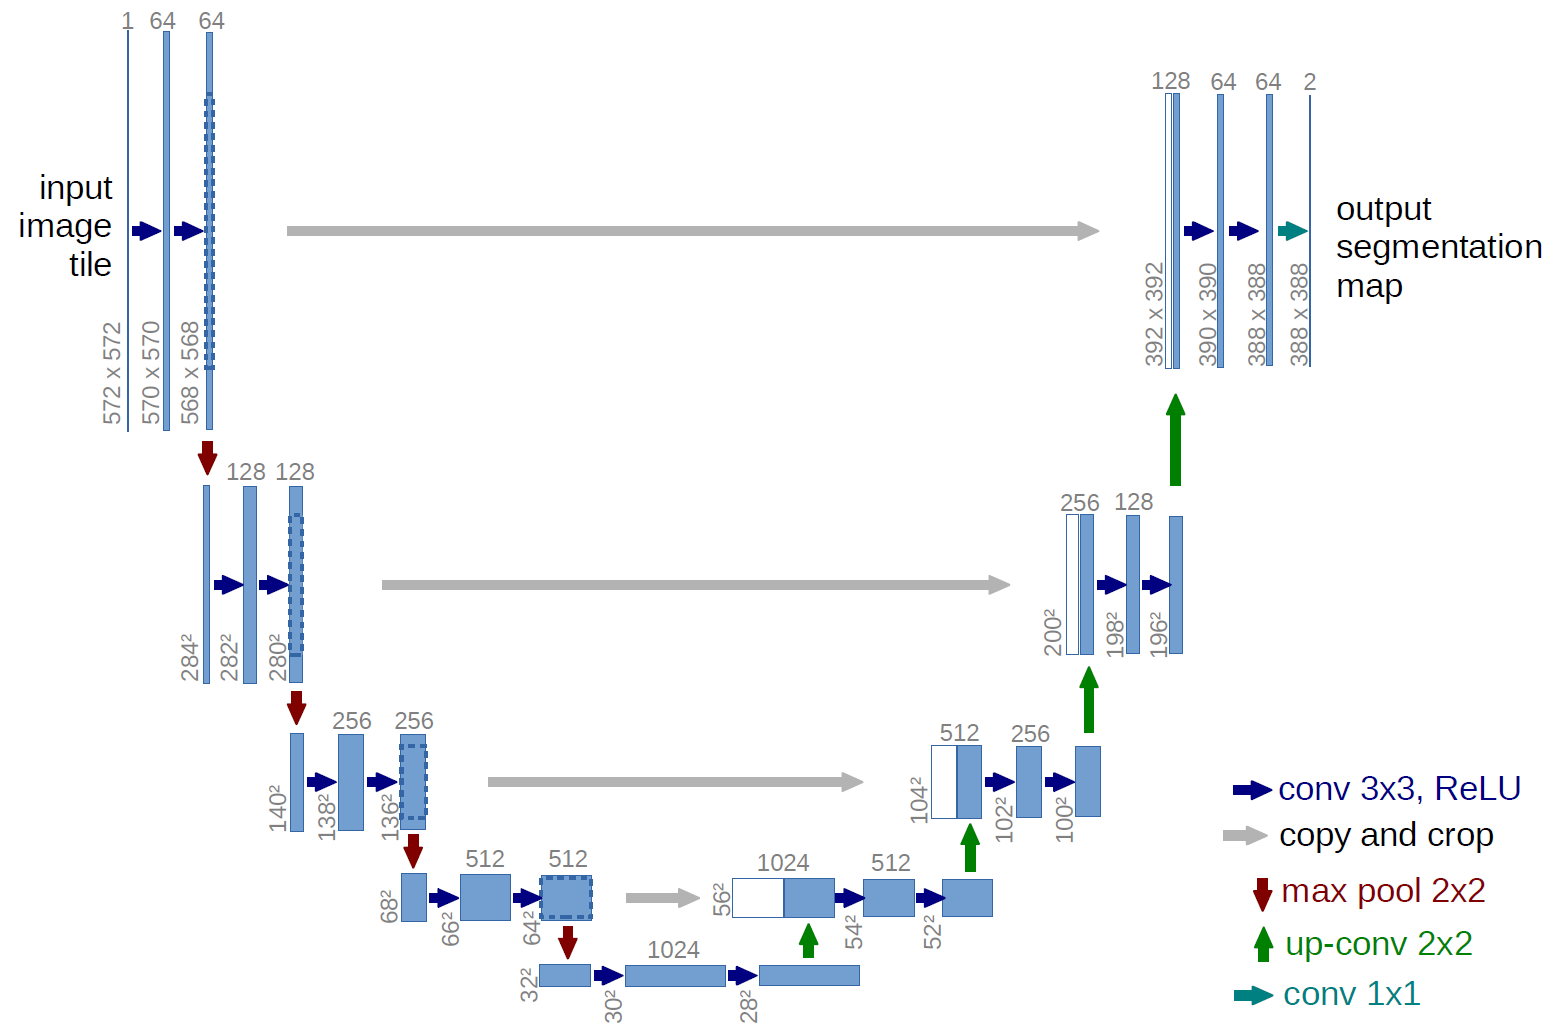
\includegraphics[width=0.8\textwidth]{Bilder/u-net-architecture.png} 
	\caption{Ursprüngliche U-Net-Architektur \cite{Ronneberger.18052015}.}
	\label{fig:u-net-architecture}
\end{figure} 


\section{Vortrainierte \ac{CNN}-Modelle} \label{sec:pretrained-backbones}

Im Folgenden wird eine Auswahl an \ac{CNN}-Modellen vorgestellt, von denen es öffentlich zugängliche,
vortrainierte Instanzen zur freien Verwendung gibt. Diese können zu Transfer-Learning-Zwecken 
genutzt werden, indem sie zum Beispiel als Teilnetz in eine \ac{CNN}-Architektur eingebaut werden 
(mehr dazu in \autoref{sec:transfer-learning}). \\ 
Die Klassifikations-Modelle sind auf dem Bildklassifikationsdatensatz \textit{ImageNet}, der über 14 Mio. Bilder 
mit 1000 Objektklassen enthält, trainiert. Der ImageNet-Datensatz ist der größte und bekannteste 
Datensatz seiner Art und ist sehr beliebt für Benchmarks und Pre-Training.

\subsection{VGG16} \label{sec:pretrained-backbones:vgg16}

\textit{VGG16} ist ein \ac{CNN}, welches 2015 von der \textit{Visual Geometry Group} vorgestellt wurde 
und zu der Zeit bahnbrechende Ergebnisse bei der Bilderklassifizierung lieferte \cite{Simonyan.04092014}. 
Inzwischen ist es ein Standard-Netz, auf welchem viele weitere Architekturen aufbauen,
um verschiedene Verbesserungen zu realisieren. 
Dadurch ist es auch sehr beliebt für Transfer-Learning. 

VGG16 besteht aus fünf Blöcken mit $3x3$-Convolution-Schichten,
gefolgt von drei Fully-Connected-Schichten. Die ersten beiden Convolution-Blöcke haben zwei Convolution-Schichten,
die letzten drei Blöcke dagegen jeweils drei. 
Jeder Convolution-Block wird gefolgt von einer Maxpool-Schicht und jeder bis auf den vorletzeten verdoppelt die Filteranzahl in den Convolution-Schichten,
beginnend bei 64 Filtern im ersten Block bis hin zu 512 Filtern in den letzten beiden Blöcken \cite{Simonyan.04092014}\footnote{\autoref{fig:vgg16-architecture} veranschaulicht VGG16.}. 

Das gesamte Netz besitzt 138 Mio. Parameter. Werden die drei Fully-Conntected-Schichten am Ende ausgelassen, 
sind es ungefähr 14,7 Mio. Parameter. 

\subsection{ResNet34} \label{sec:pretrained-backbones:resnet}

Damit Modelle mehr und feinere Features lernen können, müssen sie in der Lage sein, sehr komplexe Funktionen darzustellen. 
Das führt dazu, dass tiefere Netze auf dem ImageNet-Datensatz tendenziell bessere Ergebnisse erzeugen, als flachere. 
Hierin lag auch der Erfolg von VGG16 bzw. VGG19. Jedoch führt das einfache Vertiefen von Netzen zu dem Degredation-Problem, wonach 
flachere Netze besser performen, als tiefere, da die tieferen sehr schwer zu trainieren sind. \\
Dieses Problem adressiert \textit{ResNet} erfolgreich, indem \textit{Residual-Blocks} eingeführt werden. 
Hierdurch können mit \textit{ResNet} tiefere Netze erstellt werden als bisher, die trotzdem noch effizient trainiert werden können.
Ein Residual-Block besteht dabei aus zwei Convolutional-Layer mit einer Skip-Connection zwischen Input der ersten Layer und Output 
der zweiten Layer. Durch die Skip-Connections kann bei der Backpropagation der Gradient ungehindert rückwärts laufen, 
um so auch die flachen Layer upzudaten. So kann z.B. \textit{ResNet34} 34 trainierbare Layer haben, 
während zuvor mit VGG nur 16 bzw. 19 effektiv waren \cite{He.10122015}. 

Die Architektur ist dabei sehr simpel. Sie stellt - im Falle von ResNet34 - im Prinzip 33 Convolutional-Layer mit wiederholtem Downsampling 
und Skip-Connections zw. jeweils zwei Convoltuional-Layern, gefolgt von einer Fully-Connected-Layer dar \cite{He.10122015}\footnote{\autoref{fig:resnet34-architecture} veranschaulicht ResNet34.}.

ResNet34 hat 63,5 Mio. Parameter. Wird auf die letzte Fully-Connected-Layer verzichtet, sind es 21,2 Mio. Parameter.


\subsection{DenseNet121} \label{sec:pretrained-backbones:densenet121}

\textit{DenseNet121} wurde 2018 erstmals vorgeschlagen und wurde designed, um das Vanishing-Gradient-Problem 
zu verbessern, bessere Feature-Übertragung in tiefere Netzschichten zu ermöglichen und das Wiederverwenden von Features 
zu unterstützen, um somit die Anzahl der benötigten Parameter deutlich zu reduzieren, bei gleichbleibender Performanz \cite{Huang.25082016}.

Das Netz besteht aus mehreren sogenannten Dense-Blöcke, die wie folgt aufgebaut sind: 
Jede angegebene Convolution-Schicht besteht aus einer Batch-Normalization-Schicht mit \ac{ReLU}-Aktivierung,
gefolgt von der angegebenen Convoltuion-Schicht. Außerdem - und hier liegt die große Erweiterung des DenseNet - sind alle 
Convolution-Schichten eines Dense-Blocks mit allen nachfolgenden Convolution-Schichten des Dense-Blocks konkateniert,
anstatt nur mit dem einen Nachfolgenden, wie es zum Beispiel bei VGG16 der Fall ist\footnote{\autoref{fig:densenet121-architecture} veranschaulicht DenseNet121.}. 

DenseNet121 enthält circa 7,6 Mio. Parameter. Ohne die letzte Fully-Connected-Schicht sind es noch circa 6,9 Mio. 
Bei nur halb so vielen Parametern erreicht DenseNet121 leicht bessere Ergebnisse als VGG16 auf dem ImageNet-Datensatz 
(93\% ggü. 92\% Accuracy für ImageNet-Top5) \cite{Huang.25082016}. 


\section{Transfer-Learning mit U-Net} \label{sec:transfer-learning}

\textit{Transfer-Learning} beschreibt das Übertragen von trainierten Gewichten eines \ac{ML}-Modells auf ein anderes, 
bestenfalls ähnliches Problem und Modell. Das Modell wird dann via \textit{Fine-Tuning} verfeinert mit dem neuen Datensatz und unterschiedlichen Trainingsmethoden.
Häufig wird dafür ein Teil des Modells eingefroren, sodass sich die eingefrorenen Gewichte nicht verändern können. Dies verhindert, 
dass die bereits vortrainierten Gewichte durch die erste Trainings-Batch ruiniert und unbrauchbar werden. Eine weitere Möglichkeit ist,
mit einer sehr geringen Lernrate das gesamte Modell zu trainieren. Oft werden beide Ansätze auch verbunden.

Der Vorteil von Transfer-Learning liegt darin, dass das Training deutlich kürzer dauert, 
weil direkt mit einer höheren Genauigkeit eingestiegen wird, mit kleineren Datensätze bessere Ergebnisse erzielt werden können
 und auch insgesamt eine höhere Genauigkeit 
am Ende des Trainings erreicht wird, als bei herkömmlichem Training. Diese Effekte sind verstärkt, 
abhängig davon, wie ähnlich der Datensatz des Pre-Trainings und des eigentlichen Trainings sind \cite{Ruder.3212017}. \\
Insbesondere bei Computer-Vision ist Transfer-Learning effektiv, da bei Bildern high-level Features wie Clustering 
ähnlichfarbener Pixel oder Kantenerkennung oftmals sehr ähnlich zwischen unterschiedlichen Datensätzen ausfallen 
und damit schon vorhanden sind \cite{Ruder.3212017}. 

Für Transfer-Learning mit U-Nets gibt es verschiedene Strategien: Backbone-Netze als Encoder, 
partielles Einfrieren verschiedener Netzbereiche und direktes Trainieren mit geringer Learning-Rate.
Der Stand der Wissenschaft diesbezüglich wird im Folgenden vorgestellt. 

\subsection{Training mit Backbones} \label{sec:transfer-learning:backbones}

Im Kontext von Transfer-Learning bei U-Nets bezeichnet ein \textit{Backbone} ein etabliertes vortrainiertes \ac{CNN}, 
welches, leicht modifiziert, als Encoder für das U-Net verwendet wird. Hierbei wird der Decoder-Teil des U-Net 
symmetrisch dem Encoder nachempfunden und an passenden Stellen Skip-Verbindungen zwischen En- und Decoder eingebaut. \\
Hierdurch kann eine geeignete \ac{CNN}-Architektur für das spezifische Problem ausgewählt werden. Des Weiteren sind diese 
Modelle auf sehr großen Datensätzen, wie \textit{ImageNet}, vortrainiert öffentlich zugänglich. 

Bei der semantischen Segmentierung von medizinischen Lungen-Ultraschall-Bildern, wurden die besten Ergebnisse von einem Dice-Maß-Standpunkt aus, 
mit einem U-Net mit auf ImageNet trainierten \textit{VGG16}-Backbone erzielt. Das Vergleichsnetz, welches zuerst auf dem \textit{Salien Object}
Datensatz vortrainiert wurde, erzielte schlechtere Ergebnisse von dem Dice-Maß her, wobei allerdings das VGG16-U-Net kleine falsch-positive 
Regionen erkannte, die weit außerhalb der Ground-Truth lagen. Die falsch-positiven beim Vergleichsnetz, lagen direkt an der Ground-Truth, 
dies lässt auf eine sensitivere Kantenerkennung beim VGG16-U-Net schließen, die manchmal aber auch übersensitiv war \cite{Cheng.05.10.2021}. 

Für das Training des VGG16-U-Nets wurde der Encoder-Teil eingefroren und somit nur der Decoder trainiert. 

\subsection{Partielles Einfrieren und Training mit geringer Lernrate}

Im oben beschriebenen Problem zur semantischen Segmentierung wurde das vortrainierte Vergleichsnetz auf zwei Weisen fein-trainiert:
\begin{enumerate}
	\item Ohne Einfrieren mit einer Lernrate von $10^{-5}$
	\item und mit Einfrieren des mittleren Blocks, welcher ungefähr $14\cdot 10^6$ der insgesamt $31 \cdot 10^6$ Parameter enthielt. 
\end{enumerate}
Die 5-fache Kreuzvalidierung ergab sowohl für den besten Lauf, als auch für den durchschnittlichen Lauf, ein besseres Dice-Maß 
für das Training aller Parameter. In keinem der Fälle gab es, anders als beim VGG16-U-Net, segmentierte Regionen ohne Zusammenhang mit der Ground-Truth \cite{Cheng.05.10.2021}. 

In einem weiteren Paper wurde untersucht, welche Layer eines U-Net am besten eingefroren werden sollten, für das Fine-Tuning von medizinischen Bildern - 
zum einen von Lungen-Ultraschall-Bildern und zum anderen von Brust-Röntgen-Aufnahmen. 
Hier wurde wieder mit dem \textit{Salien Objetcs} Datensatz vortrainiert. Dann wurden für beide Anwendungsfälle folgende Tests durchgeführt: 
\begin{enumerate}
	\item Einfrieren der linken Hälfte (Encoder) des Netzes,
	\item Einfrieren der rechten Hälfte (Decoder) des Netzes,
	\item gesamtes Netz, bis auf den ersten Block eingefroren und dann nach jeweils fünf Epochen sukkzessive weitere Blöcke freigeben und
	\item dasselbe allerdings von hinten nach vorne.
\end{enumerate}
Für die Röntgenaufnahmen gab es keine Unterschiede, wobei der Dice-Score hier allerdings auch bei $0.98$ lag. 
Für die Ultraschallbilder lieferte Methode (1) die schlechtesten Ergebnisse (Dice: $0.72$), gefolgt von Methode (2) (Dice: $0.80$) 
und gleichermaßen (3) und (4) (Dice: $0.82$), wobei (3) deutlich schneller konvergierte \cite{Amiri.19.02.2020}. \\ 
Es ist ersichtlich, dass die Methodik beim Fine-Tuning, abhängig vom Datensatz, einen erheblichen Einfluss 
auf die abschließende Performanz des Modells haben kann und stets berücksichtigt und gegen Alternativen abgewogen werden sollte,
um beste Ergebnisse zu erzielen. Die vorgestellten Methodiken können später genutzt werden, 
um eine Transfer-Learning-Methode für das Problem der Radwegerkennung zu konzipieren. 


\section{Aktueller Stand bei der Straßendetektion}

Die Erkennung von Fahrradwegen soll auf der bereits existierenden Straßenextraktion aus Satellitenbildern aufbauen.
Hierfür werden vorhandene Datensätze für Straßen vorgestellt. 
Im Anschluss werden auf den aktuellen Stand und Benchmark-Optionen eingegangen.

\subsection{Datensätze} \label{sec:road-detection:roads-data}

Im Folgenden sind alle relevanten Datensätze zur Straßenerkennung aus Luftbildern aufgeführt. 
Eine Auswahl der später zum Pre-Training verwendeten Datensätze findet im \autoref{sec:pre-training-roads} statt.\\
Ein Testdatensatz ist hierbei ein meist sehr kleiner Datensatz, der ausschließlich zum Testen und Bewerten eines bereits 
trainierten Modells verwendet werden soll. Im Rahmen der Straßenerkennung ist dies besonders relevant, 
da sich unterschiedliche Städte in unterschiedlichen Ländern und Kulturen stark unterscheiden können, 
während die Trainingsdaten meist nur aus einer Stadt, die in sich ein eher homogenes Bild aufweist, bestehen.
Der Testdatensatz soll also die Generalisierungsfähigkeit des Netzes testen, um zu sehen,
ob das Modell, das bspw. auf einem Datensatz einer modernen amerikanischen Stadt trainiert wurde, 
auch auf Bildern einer mitteleuropäischen Altstadt funktioniert. Deswegen ist es wichtig, 
dass keine Bilder des Testdatensatzes im Training verwendet werden. 

% Bei den letzten Datensets zu Toronto, Vaihingent und Potsdam handelt es sich um Testdatensätze. 
Beim \textit{Massachusetts Roads Dataset} liegen $1171$ Luftaufnahmen aus dem Gebiet Massachusetts vor.
Jedes der Bilder besteht aus $1500\times 1500$ Pixeln, was einer Fläche von $2.25 km^2$ entspricht.
Die gesamte Abdeckung sind $2600 km^2$ bestehend aus städtischer und ländlicher Gegend.
Der Split erfolgt im Verhältnis $95:1:4$. 
Über den Split wird sichergestellt, dass keine Durchmischung der Test- und Validierungsdaten mit den Trainingsdaten erfolgt und die Bewertung des Netzes verfälscht wird.
Es gibt also $1108$ Trainings-, $14$ Validierungs- und $49$ Testbilder.
Die Zielbilder sind über eine Rasterung der Straßenmittellinien aus dem OpenStreetMap-Projekt generiert worden.
Die Liniendicke der gelabelten Straßen beträgt $7 px$ und ist ungeglättet, da hiermit bessere Ergebnisse erzielt worden sind \cite[S.~85f]{.06.04.2014}.
Der Zuschnitt der Bilder sorgt teilweise für einen hohen Anteil weißer Stellen in den Bildern.

Das \textit{Buffalo Roads Dataset} ist als zusätzliches Testset für das Massachusetts Roads Dataset zu sehen.
Hintergrund ist die Überprüfung des Netzes mit Daten aus einem anderem Gebiet unter anderen Bedingungen.
Es besteht lediglich aus 30 Orthophotos ($5:5:20$) mit einer Größe von $609\times 914$ und einer Auflösung von $1 \frac{px}{m^2}$.
Die Generierung der gelabelten Daten erfolgt analog zum Massachusetts Road Set über OpenStreetMap.
Größter Unterschied ist die Verdeckung von Straßen durch Bäume \cite[86-88]{.06.04.2014}.

\textit{LandCover.ai} kann für die Erkennung von Gebäuden, Waldgebieten, Gewässern und Straßen verwendet werden.
Die Aufnahmen stammen aus Polen und Zentraleuropa in einer Größe von $21627 km^2$.
$33$ Orthophotos haben eine Auflösung von $25 \frac{cm}{px}$ mit $9000\times 9500$ Pixeln, $8$ Bilder von $50 \frac{cm}{px}$ mit $4200 \times 4700$ Pixeln \cite{.20.04.2022}.
Die Bilder sind hand-annotiert und beinhalten einen großen Anteil an ländlichen Gebieten.

Mithilfe des \textit{Deep Globe Road Extraction Datasets} können in Kathastrophgebieten Informationen über Karten und Zugänglichkeitsmöglichkeiten für die Krisenbewältigung gesammelt werden.
Der Datensatz besteht aus $6226$ Satellitenbildern in RGB mit einer Größe von $1024\times 1024$.
Die Auflösung der Aufnahmen beträgt $50 cm$.
Mit $1243$ Validierungs- und $1101$ Testdaten ist der Split in Training, Validierung und Test zu $73:15:13$ erfolgt.
Der hohe Aufwand zur Erstellung der Labels führt zu Ungenauigkeiten, insbesondere in ländlichen Regionen. 
Kleine Straßen innerhalb von Landwirtschaftsflächen sind bewusst unbeschriftet geblieben.
Die Bilder sind ursprünglich über Thailand, Indonesien und Indien mit je $19584\times 19584$ Pixeln aufgenommen worden.
Insgesamt entspricht es einer Fläche von $2220 km^2$ \cite{Ashwath.10.11.2020}.

Mit finanzieller Unterstützung des Chesapeak Bay Programms wurde ein Datensatz \textit{Land Cover} zur Landnutzung und Bodenbedeckung erstellt.
Es lassen sich Einblicke in die Landschaft und die Verwaltung der Regionen gewinnen.
Das Einzugsgebiet umfasst $250.000km^2$ mit einer Auflösung von $1m$. 
Damit handelt es sich bei diesem Datensatz um den größten bei der Analyse von der Landnutzung im Vergleich zur Bodenbedeckung \cite{ChesapeakeConservancy.02.06.2022}.

Bei den nachfolgenden drei Datensätzen handelt es sich um Testdatensätze.
Das \textit{Toronto Dataset} umfasst $1,45km^2$ im Umkreis der Stadt Toronto in Canada. 
Darin enthalten sind ca. $1 km$ Straßen mit einer Bodenauflösung von $15cm$. 
Zusätzlich werden Laserscanner mit $6 \frac{points}{m^2}$ bereitgestellt.
Im Datensatz ist eine hohe Varianz bezüglich der Gebäudehöhe, Struktur der Dächer und verschiedener Straßen vorzufinden.
Der Testbestand kann für die Überprüfung von Objektextraktion und Gebäuderekonstruktionstechniken in zwei weitere Teilgebiete unterteilt werden.
Für Straßen können alle Testdaten verwendet werden.
Die Labels sind manuell mithilfe von CloudCompare erstellt worden \cite{Englich.06.10.2022b,Tan.2020}.

Der Testdatensatz \textit{Vaihingen/Enz} besteht aus einer Untermenge der Daten, welche für einen Test von digitalen Luftbildkameras verwendet wurden.
Er ist in drei Testgebiete für verschiedene Objektklassen und in einen größeren Bereich für das Überprüfen von Straßenextrakion aufgeteilt, wobei die drei Gebiete hier mit inbegriffen sind.
Die einzelnen Gebiete sind in verschiedene Kategorien unterteilt: Hochhäuser, Wohngebiete mit kleineren Einfamilienhäusern und Innenstadt mit dichter Bebauung.
Die Bodenauflösung beträgt $8cm$ \cite{Englich.06.10.2022b}.

Für die Stadt \textit{Potsdam} gibt es einen ähnlichen Datensatz. 
Dieser zeigt eine typsiche Altstadt mit großen Gebäudeblöcken, kleinen Straßen und einer dichten Besiedelung.
Die \ac{GSD} beträgt $5cm$.
Zur Vermeidung von Randbereichen ohne Daten, sind zentrale Ausschnitte verwendet worden.
Übrig gebliebene Datenlücken wurden interpoliert \cite{Englich.17.11.2022, Englich.17.11.2022b}.

\subsection{Aktueller Stand und Benchmarks} \label{sec:state-of-the-art-roads} % ...der straßen detection

Die aktuellen State-Of-The-Art-Methoden zur Extraktion von Straßen aus Satelliten- und Luftbildern verwenden 
alle Computer-Vision mittels \acp{CNN} und dabei ausschließlich Netze aus der U-Net-Familie - also angepasste, 
erweiterte, abgeänderte U-Nets \cites{C.Henry.2021, Constantin.2018, Kamiya.2018, Yerram.2022}. \\
Dies liegt vor allem daran, dass das U-Net, welches ursprünglich für biomedizinische Bilder entworfen wurde, 
genau die Probleme adressiert, die auch beim Segmentieren von Straßen auf Luftbildern auftreten. 
Wie auch in medizinischen Bildern leiden die Luftbilder-Datensätze häufig unter großer Klassen-Imbalance 
und unter ähnlichen Annotationsfehlern. Außerdem haben viele medizinische Bilder und Luftbildaufnahmen von Straßen 
ähnliche Topologien. Komplexere Architekturen zur semantischen Segmentierung, wie zum Beispiel solche 
für Bodenaufnahmen-Datensätze (vgl. KITTI \cite{Geiger.2013}) erreichen nicht die Performance von U-Nets bei 
Luftbild-Benchmarks \cite{C.Henry.2021}. \\
Weiter wird die Extraktion von Straßen aus Satelliten- bzw. Luftbildern zumeist in zwei Phasen eingeteilt: 
\begin{enumerate}
	\item das Erstellen einer binären Maske zu den Luftbildern mittels semantischer Segmentierung, 
	welche die Straßen pixelweise induziert, 
	\item das Extrahieren eines topologischen Graphens, welcher die Straßen-Zentrumslinien beschreibt.   
\end{enumerate}
Schritt (1) wird dabei zumeist von U-Net-Derivaten behandelt, wobei es allerdings auch Vorschläge von Netzen gibt, 
die direkt Schritt (2) ausführen \cite{C.Henry.2021}.
Im Folgenden wird weiter Schritt (1) betrachtet.   

Der Vergleich von unterschiedlichen Netzen, Papern und Ergebnissen zur Straßenerkennung ist häufig erschwert, 
da es trotz gleicher Bewertungsmaße wie Dice oder \ac{IoU}, zwei unterschiedliche gängige Kodierungen gibt:
\begin{enumerate}
	\item Das verwendete \ac{CNN} hat je Input-Neuron bzw. -Pixel $p$ genau ein Output-Neuron $o_p$, welches den jeweiligen Input-Pixel $p$
	als Straße identifiziert, genau dann, wenn der Wert des Output-Neuron $o_p$ einen gewissen Grenzwert $l$ überschreitet ($o_p > l$), 
	ansonsten ($o_p \leq l$) gilt der Pixel $p$ \textit{implizit} als Nicht-Straße, bzw. \textit{Hintergrund}. \\
	In diesem Fall stellt ein korrekt als Hintergrund klassifizierter Pixel ein wahr-negatives Ergebnis dar. 
	Wahr-Negative werden von Dice, bzw. \ac{IoU} allerdings nicht berücksichtigt (vgl. \autoref{eq:f1} und \ref{eq:iou-binary}).
	Ein so klassifizierter Pixel ändert also nichts an dem Score. Es werden nur Straßen betrachtet, nicht aber der Hintergrund.    
	\item Das verwendete \ac{CNN} hat je Input-Neuron bzw. -Pixel $p$ \textit{zwei} Output-Neuronen $\mathbf{o_p} = (o_{p_S}, o_{p_H})$, 
	wobei dies eine One-Hot-Kodierung von Punkt (1) darstellt. 
	Ein Hintergrund-Pixel wird nun \textit{explizit} als solcher klassifiziert. 
	Dies ändert allerdings die Berechnungsgrundlage von Dice und \ac{IoU} erheblich, da diese nun (zumeist) als Mittelwert 
	der Scores zu $o_p{_S}$ und $o_p{_H}$ berechnet werden. Hierdurch fließen die zuvor unberücksichtigten wahr-negativen 
	Hintergrundpixel als wahr-postive in den Dice- bzw. \ac{IoU}-Score ein. Die Verzerrung wird noch verstärkt, 
	da eine starke Imbalance zwischen Straßen- und Hintergrundpixel herrscht, wodurch der Dice-/\ac{IoU}-Score bei 
	der One-Hot-Kodierung viel mehr eine Aussage darüber trifft, wie viele Hintergrundpixel, von denen es ja viel mehr gibt,
	richtig klassifiziert wurden. Die so erzielten Dice-/IoU-Werte sind hier rein numerisch deutlich höher. 
\end{enumerate}

Im Weiteren werden aktuelle Ergebnisse zu den Massachusetts- und Deep-Globe-Datensätzen vorgestellt, 
um zu Ermitteln, was für diese Datensätze gut funktioniert, sodass diese state-of-the-art Erkenntnisse beim 
späteren Entwurf eines oder mehrerer Netze zum Erkennen von Fahrradwegen (s. \autoref{sec:architecture}) 
genutzt werden können. Die beiden Datensätze sind für die Literaturrecherche ausgewählt, 
da sie sehr häufig als Benchmark zum Erkennen von Straßen genutzt werden, es dazu sehr viel Literatur und 
Forschung gibt und da beide Datensätze sich stark unterscheiden, soweit das im Rahmen der Straßenerkennung möglich ist. 
Haben die State-Of-The-Art-Lösungen trotz des starken Unterschieds der Datensätze ähnliche gut funktionierende
Komponenten, stärkt das die Annahme, dass diese Komponenten auch für das Erkennen von Radwegen nützlich sein könnten. \\   
\autoref{tab:basline-benchmarks} zeigt Resultate zum Massachusetts- und Deep-Globe-Datensatz von sogenannten \textit{Basline}-Modellen.
Hierbei handelt es sich um verschiedene Architekturen, die allerdings nicht extrem auf den jeweiligen Datensatz optimiert sind,
was die Hyper-Parameter oder manche Architektur-Anpassungen angeht. Ein Beispiel dafür wäre das Ausprobieren von verschiedenen (Kompositions-)Kostenfunktionen. 
Mit den Baseline-Resultaten können diese Modelle zu Vergleichszwecken verwendet werden 
und es bestehen Daten zu mehreren Benchmarks \cite{C.Henry.2021}.

\begin{table}
	\centering
	\begin{tabular}{l|l|l|l|l}
		\multirow{2}{*}{Model} & \multicolumn{2}{c|}{Massachusetts} & \multicolumn{2}{c}{Deep Globe}  \\
		& Dice & IoU & Dice & IoU \\
		\midrule
		DeepLabv3+* & 69,35 & 52,95 & 75,19 & 59,65 \\
		D-LinkNet50 & 71,01 & 54,90 & 74,04 & 58,12 \\
		U-Net* & 71,91 & 55,92 & 76,82 & 61,97 \\
		Res-U-Net50 & 72,74 & 56,93 & 78,62 & 64,55  \\
		Dense-U-Net-121 & \textbf{73,03} & \textbf{57,12} & \textbf{79,19} & \textbf{65,13}  \\
	\end{tabular}
	\caption{Baseline-Resultate verschiedener Modelle auf dem Massachusetts- 
	bzw. Deep-Globe-Datensatz in Prozent, aufsteigend sortiert. Nicht one-hot-kodiert. * nicht vortrainiert. \cite{C.Henry.2021}.}
	\label{tab:basline-benchmarks}
\end{table}

\autoref{tab:optimized-benchmarks} zeigt hingegen die top-drei optimierten Modelle, die derzeit die Leaderboards 
des jeweiligen Datensatzes anführen. Alle hiervon sind U-Net-Derivate.
Mit der Modell-Optimierung kann \textit{Dense-U-Net-121} aus \autoref{tab:basline-benchmarks} beispielsweise beim Massachusetts-Datensatz 
bis zu 66,61\% erreichen, anstelle von den 57,12\% wie im Baseline-Fall. 
Dense-U-Net-121 ist dabei ein U-Net mit einem vortrainierten DenseNet121 als Backbone \cite{C.Henry.2021}. \\
Im Falle vom RDRCNN (Refined Deep Residual Convolutional Neural Network), konnte die große Verbesserung erzielt werden,
indem das U-Net so angepasst wurde, dass die Encoder-Blöcke mit Residual-Blöcken\footnote{Zwei Convolutional-Layer bei dem eine Skip-Connection zwischen Input der ersten und Output der zweiten Schicht besteht (s. \autoref{sec:pretrained-backbones:resnet}).} 
ersetzt wurden und der Bottleneck-Block
um Dilation erweitert wurde \cite{Gao.2019}. 
Beim EOSResUNet wurden ebenfalls die Encoder-Blöcke mit Residual-Blöcken ersetzt und zusätzlich nach \ac{IoU} statt nach Dice oder \ac{BCE} optimiert \cite{O.Filin.2018}. \\
Die besten Netze beider Datensätze haben die Gemeinsamkeit der U-Net-Struktur, wie auch die Residual-Blöcke (bzw.
sogar Dense-Blöcke, was als eine Erweiterung der Residual-Blöcke aufgefasst werden kann). 
Diese Informationen können zur Konzeption eines Netzes zur Radwegerkennung verwendet werden.  

\newcommand*\rot{\rotatebox{60}}

\begin{table}
	\centering
	\begin{tabular}{l|lll|lll}
		& \multicolumn{3}{c|}{Massachusetts} & \multicolumn{3}{c}{Deep Globe}  \\
		\rot{Model} & \rot{RDRCNN} & \rot{\begin{tabular}[x]{@{}c@{}}Dense-U-Net-\\121\end{tabular}} & \rot{WRAU-Net} & \rot{EOSResUNet} & \rot{D-LinkNet} & \rot{\begin{tabular}[x]{@{}c@{}}U-Net-like\\ResNet34\end{tabular}} \\
		\midrule
		IoU & \textbf{67,10} & 66,61 & 64,58 & \textbf{65,60} & 64,12 & 64,00 
	\end{tabular}
	\caption{Optimierte Resultate verschiedener Modelle auf dem Massachusetts- 
	bzw. Deep-Globe-Datensatz in Prozent, absteigend sortiert von links nach rechts. Nicht one-hot-kodiert. \cite{C.Henry.2021}.}
	\label{tab:optimized-benchmarks}
\end{table}